\section{Introduction}
Over the past decade, significant progress has been made in the development of Advanced Driver Assistance Systems (ADAS) and autonomous driving technologies. 
These technologies have become increasingly intelligent, with autonomous driving progressing beyond level 2 toward level 3 of driving automation as defined by the Society for Automotive Engineers (SAE) \cite{sae20213016}. 
% This means that there is a growing amount of time during which the driver is not actively involved in the driving task. 
However, the mass production of technology surpassing level 3 of driving automation is not yet available, primarily due to three main reasons as follows: safety, interpretability, and ride comfort.
In level 3, the system must be liable for all potential accidents that occur during its operation, making safety a top priority.
To ensure safety, it is crucial to redundantly acquire various perception information.
Claiming responsibility also necessitates providing justifications for the system's perception information, highlighting the importance of ensuring interpretability of the perception information is also essential.
In addition to quantitative perception information such as distance to preceding vehicles, relative velocity, and time to collision (TTC), more intuitive information is needed.
Furthermore, ride comport is a significant issue that should not be overlooked in the widespread adoption of ADAS and autonomous driving technology, with motion sickness being a crucial concern \cite{diels2016self, iskander2019car}.
Some even refer to it as ``autonomous car sickness'' \cite{iskander2019car}.
Motion sickness arises from conflicts between sensory inputs, where the detected motion information deviates from the expectations based on past experiences during autonomous driving \cite{reason1975motion,reason1978motion}.
In other words, autonomous driving systems need to mimic human driving behavior to mitigate motion sickness and enhance ride comport.

To address these challenges, we propose a new method for detecting driving vehicles and their brake light status.
Brake light status information is crucial for multiple drivers to ensure safety on the road.
Human drivers adjust their driving patterns based not only on distance and relative velocity but also on the brake light status of neighboring vehicles. 
Autonomous driving systems aiming for enhanced safety should not overlook this fundamental information.
Additionally, brake light status is particularly intuitive and possesses effective interpretability when communicating with humans.
While distance, relative velocity, and TTC may provide clearer information among machines, brake light status information offers a more intuitive understanding.
For example, when following a leading vehicle, a machine can maintain a much tighter gap with the leading vehicle by utilizing a combination of distance, relative velocity, and TTC than human drivers.
However, since human drivers normally can not grasp the intricacies of distance, relative velocity, and TTC as tightly as the machines do, when the brake light of the leading vehicle illuminate, human drivers stop the accelerate and prepare for possible deceleration of the leading vehicle.
Therefore, driving technology that considers brake light status as well can be more persuasive to humans.
Furthermore, considering the brake light status in ADAS can improve ride comfort \cite{pirhonen2022predictive}.
By acquiring redundantly interpretable perceptual information, including brake light status, ADAS or autonomous driving systems can drive in a more human-like manner, ultimately reducing sensory conflicts and alleviating motion sickness.


% There are various theories explaining the causes of motion sickness, but this study focuses specifically on the sensory conflict theory. 
% According to this theory, motion sickness occurs due to a conflict between sensory inputs, where the detected motion information deviates from the expectation based on past experiences \cite{reason1975motion,reason1978motion}. 
% For instance, in the case of adaptive cruise control (ACC), which intelligently follows the preceding vehicle by considering factors such as distance, relative velocity, and time to collision (TTC), many drivers and passengers experience discomfort and motion sickness due to the discrepancy between their previous experiences and the system's actions. 
% One of the main causes of this discrepancy is the system's failure to consider the operation of the preceding vehicle's brakes. Humans adjust their following patterns based not only on the distance and relative velocity but also on the operation of the preceding vehicle's brakes. 

\begin{figure}[]
    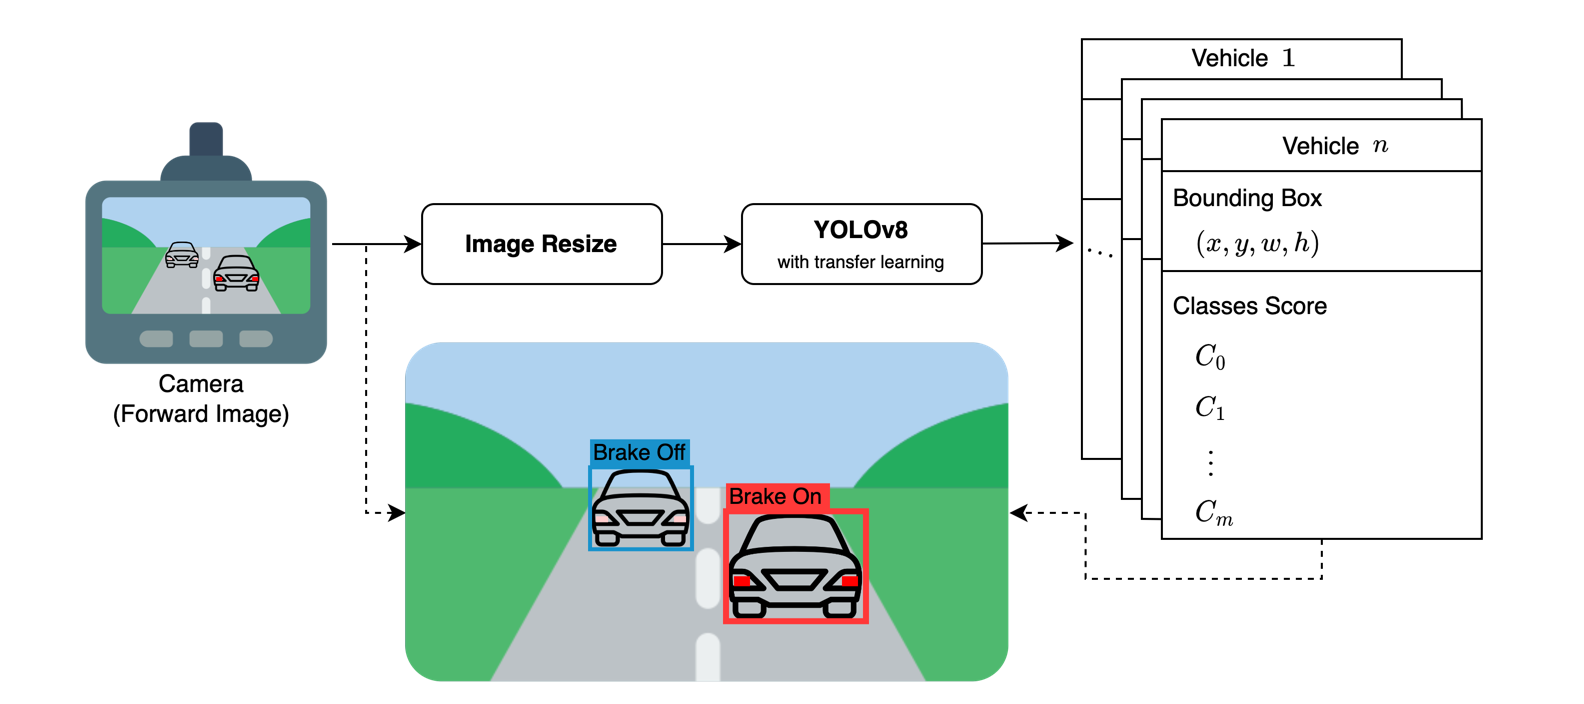
\includegraphics[scale=0.5]{fig/workflow.png}
    \caption{Workflow of the proposed one-stage brake light detection network. The solid line arrows represent the flow of data for inference purposes, while the dashed line arrows represent the flow of data for visualization purposes.}
    \label{fig:workflow}
\end{figure}

In this paper, we propose a one-stage neural network that detects brake lights of preceding vehicles, taking into account the trade-off between inference time and accurate detection performance. 
The proposed network is based on YOLOv8 \cite{YOLOv8}, the latest version of the popular one-stage object detection network as shown in Figure \ref{fig:workflow}.
We leverage transfer learning to train the network for the task of detecting driving vehicles and brake light.
% Existing research on brake light detection utilizing computer vision or artificial neural network techniques exists, but they typically employ multi-stage architectures of two or more stages, neglecting the inference time.

To train the network, we collected over $11,000$ real-world driving images and manually annotated the driving vehicle and brake light status for each image.
This dataset was used for transfer learning with YOLOv8. 
We conducted transfer learning and evaluated the performance of the models in terms of model size, brake light status, and ambient lighting conditions.
The real-time performance of the trained models was verified using an edge device, the Nvidia Jetson Nano, installed in the driving vehicle.
The Jetson Nano is one of Nvidia's platform series designed for embedded applications of neural networks.
Among the product line, it stands out as the smallest form factor with the lowest power consumption, making it widely used for real-time inference experiments, especially in resource-constrained environments \cite{assunccao2022real}.
This verification allowed us to assess the model's ability to make predictions in real-time while considering computational efficiency.

The main contributions in this study can be described as follows:
\begin{itemize}
    \item Proposal of a one-stage network for detecting the brake light status of vehicles in the forward image during driving. The proposed network takes a single image as input and provides bounding boxes for all vehicles in the image, along with the detection of whether their brake light is on or off. 
    \item Introduction of a dataset specifically designed for the task of driving vehicle and brake light status detection. The dataset comprises over $11,000$ real-world driving images captured under various conditions, including day, night, and tunnel scenarios. Each image in the dataset is annotated by experts with vehicle bounding boxes and brake light status.
    \item Fine-tuning of the proposed detection network based on YOLOv8 using the introduced dataset. The trained model demonstrates high detection performance, and its real-time performance on an edge device is validated.
\end{itemize}

The remainder of this paper is organized as follows:
Section \ref{sec:related} provides an overview of related works on brake light status detection. 
Section \ref{sec:proposed} discusses the proposed detection network and dataset used for transfer learning.
Section \ref{sec:experiments} presents the methodology for transfer learning and analyzes the evaluation results.
Section \ref{sec:conclusions} concludes the work and outlines potential future research directions. 